\subsection{Introduction}
The term "brain (or neural) oscillations" refers to the rhythmic and/or repetitive electrical 
activity generated spontaneously and in response to stimuli by neural tissue in the central 
nervous system. The importance of brain oscillations in sensory-cognitive processes has become 
increasingly evident. This chapter will focus on some questions:
\begin{itemize}
    \item What does a neural oscillation consist of and how does it originate?
    \item What are the (main) roles of brain oscillations?
    \item How do we observe and characterize a brain oscillation?
\end{itemize}

\subsection{Neuronal Geometry and Architecture}
By looking at the extracellular field potentials, brain signals are strongly dependent on the 
geometry of the system (e.g., the hippocampus has a very different geometry with respect to 
the subthalamic nuclei). Based on the geometry and the architecture of the system, the signals 
could be very different.
\begin{itemize}
    \item Much of the signals taken into account are coming from \textbf{pyramidal cells}, because they have a very 
    specific geometry and orientation that create aligned electrical dipoles, which generate very strong 
    electrical field potentials.
    \item There are also \textbf{spherically symmetric neurons} (e.g., thalamocortical cells) which have a circular 
    geometry with dendrites of relatively equal size in all directions that somehow reduces the possibility of 
    having very synchronized field potentials.
\end{itemize}

\subsection{EEG and MEG}
Electroencephalography (EEG) and Magnetoencephalography (MEG) are the main classical techniques for recording 
non-invasively the electrical activity from the human brain. These two techniques can be combined with systems 
that record both the electrical field and the magnetic field, but, in general, they record two different aspects 
of the same event: there is a current that travels along the axons of the dendrites generating an electrical 
field that is summed among many cells and finally reaches the sensors. Depending on the physical variable that is 
taken into account, an EEG or a MEG can be recorded.
\begin{itemize}
    \item The EEG records the electrical field and, for this reason, the unit of measurement is volts (typically 
    microvolts, \(10^{-6}\,V\)).
    \item The MEG records the magnetic inducted component in a static magnetic field where the head of the person is 
    immersed on. The unit of measurement is tesla (typically femtotesla, which is \(10^{-15}\,T\)).
\end{itemize}
One of the major difference is the fact that the two systems are very different in terms of acquisition systems: EEG 
is composed by sensors placed on the scalp and wires (one for each electrode) connected to an amplifier, because 
electrical fields have a power that needs to be amplified, while MEG requires dedicated and specially built rooms and 
more intensive and expensive maintenance.
One drawback of the MEG is the fact that the coils are fixed, and so, if the subject moves his head, there is a 
a magnetic induction even though the current is not travelling, and data are completely useless.\\
One of the main reason for acquiring and looking at MEG instead of EEG is the fact that magnetic fields pass through the 
skull and scalp, whereas the electrical fields are volume conducted through these tissues, which decreases 
signal-to-noise ratio at higher frequencies (performing a low-pass filtering). For this reason, MEG signals have a 
larger power in terms of spatial resolution (better localization power), and this could be useful, for instance, 
for clinical purpose, as for studying epilepsy.

\subsubsection{Origin of EEG Signal}
This technique is not so different from what has been said regarding local field potentials, but it has one more 
problem: the sensors are not located into the brain but outside, and so the signal has to travel all the distance 
from the source up to the electrodes. EEG is the synchronized synaptic activity in populations of cortical neurons 
closer to the electrode, and it performs a spatial integration (net sum at the electrode).
What is the problem of the spatial integration? There is a difference governed by the \textbf{orientation} of the neurons.
\par\medskip
Electrodes detect the sum of positive and negative charges in their vicinity. In the case where an electrode is 
equidistant from both \textit{source} (region of positive charge) and \textit{sink} (region of negative charge) 
of a dipole, the electrode will measure a net neutral; so, an electrode can only detect dipoles when it is  
closer to either the positive or negative end of the dipole. This means that two major types of dipoles are 
measurable in EEG: tangential dipoles, which are oriented perpendicular to the surface (first figure), and radial 
dipoles, which are oriented parallel to the scalp surface (second figure). Dipoles have a positive and negative side, 
and therefore will produce both a positive deflection and a negative deflection at different regions of the scalp.
\begin{figure}[H]
    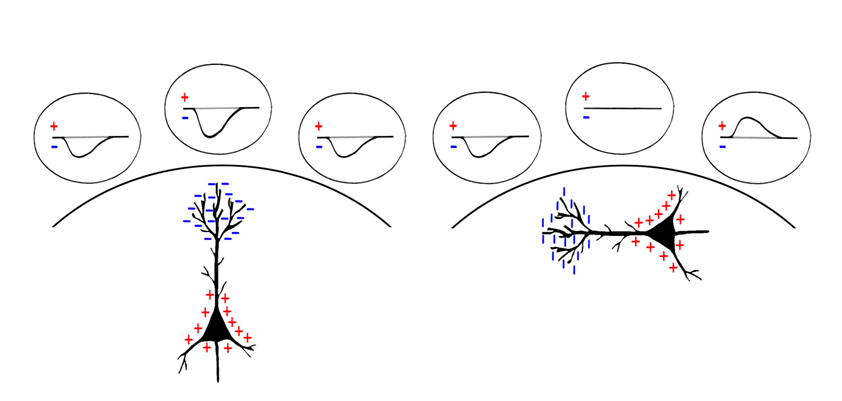
\includegraphics[scale=0.55]{10_1}
    \centering
\end{figure}
\par\medskip
A single neuron's dipole is too small to be measured as far away as the scalp. However, because electrodes detect the 
sum of charges in their vicinity, the dipoles from multiple neurons in a region will sum together. The sum of many 
individual dipoles in an area is measurable as a single dipole whose magnitude reflects the number of neurons whose 
dipoles are summing together. However, because electrodes will measure the sum of both the positive and the negative 
ends of dipoles in the brain, in order to produce a measurable (nonzero) signal, neurons must be both arranged in a 
\textit{parallel manner}, and they must be \textit{synchronously active}. 
\begin{figure}[H]
    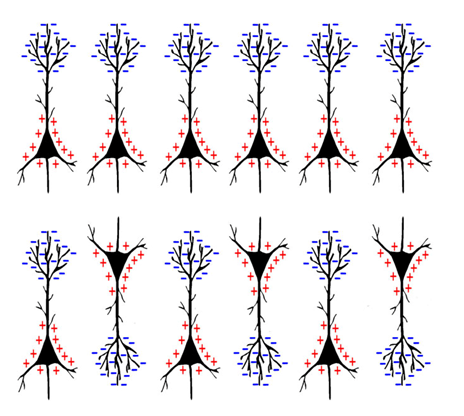
\includegraphics[scale=0.45]{10_2}
    \centering
\end{figure}
The parallel arrangement is necessary to produce a measurable 
dipole because, if the neurons are all arrayed in the same orientation, then their signals can sum to form a larger 
signal. In any other configuration, the individual dipoles' positive and negative ends will sum and cancel each other 
out. The synchronization of activity is necessary in order to yield a net charge on the scalp-facing side of the 
dipole sheet, rather than charges cancelling each other out, and also to have a signal large enough to be measured.
\par\medskip
Finally, given the fact that the electrical field moves in space for reaching the sensors (and this phenomenon can 
be called \textbf{Volume Conduction}), the signal reaches at least the outer skull layers. If there is not a layer 
that facilitates the passage of ions, it is not possible to record anything. At this purpose a conductive gel can 
be used, in order to allow the passage of ions from the sources up to the sensors.
\begin{figure}[H]
    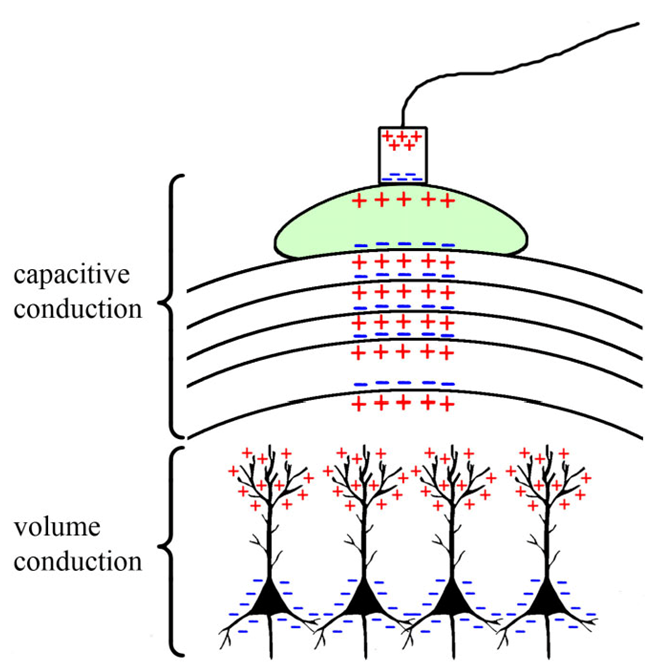
\includegraphics[scale=0.40]{10_3}
    \centering
\end{figure}

\subsubsection{EEG (Simplified) DAQ}
Which systems are capable of acquiring the data? In the following it is possible to see a simplified model of 
the EEG acquisition system:
\begin{itemize}
    \item The first element is the \textbf{Sensor}, that has some sort of resistance (\(R_1\)), referred to 
    the scalp.
    \item Then there is a \textbf{Cable}, that is used to connect the sensor to the amplifier. 
    The resistance is \(R_2\).
    \item The last part is the \textbf{Amplification System}, with its resistance \(R_3\).
\end{itemize}
\begin{figure}[H]
    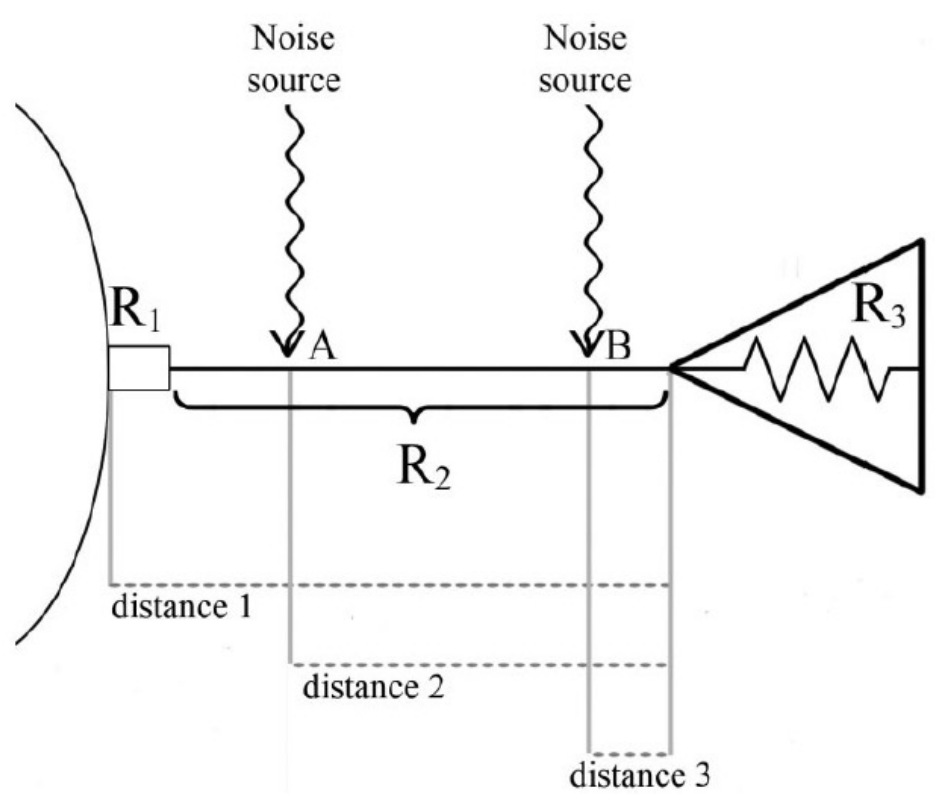
\includegraphics[scale=0.30]{10_4}
    \centering
\end{figure}
For the reasons seen before, \(R_1\) must be as low as possible to permit the ions to reach the sensors. Also the 
resistance of the cable (\(R_2\)) needs to be very small, in order not to have any loss of the signal. What can be 
said about \(R_3\)? It should be very large, compared to \(R_1\) and \(R2\), in particular it must be orders of 
magnitude larger than the sum of the two. When the data is acquired, the voltage that is considered is the one 
incident to \(R_3\); the signal that reaches \(R_3\) is composed by the activity incident to \(R_1\) and the noise 
added from the sources \(A\) and \(B\). \(R_1\) and \(A\) are very close to each other, and they decay of the same 
amount reaching \(R_2\); the very huge different (if \(R_3\) is very small) is that the largest fraction of the recorded 
activity is not dependent on the signal but is mainly noise. \\
In the other sense, if there is a very huge amplifier resistance, what happens is that the potential will be largely equally 
dependent from the noise and the signal itself: this, somehow, allows to have a better signal-to-noise ratio.
More modern acquisition systems tend to improve these two factors:
\begin{itemize}
    \item Increase of \(R_3\).
    \item Reduce the distance from the amplifier and the sensors. A large part of the modern systems has a pre-amplification, 
    that directly attaches to the sensors.
\end{itemize}

\subsubsection{EEG Principles and Good Practice}
What needs to be monitored to get the best possible data?
\begin{enumerate}
    \item \textbf{Care in Collection}: it is necessary to pay attention on the amount of gel introduced, depending on the quantity 
    of channels on the top of the head and also depending on the size of the head. If the electrodes are very close to each other, 
    the conductive gel can create the so called \textit{bridge} that attaches two sensors together.
    \item \textbf{Care in Interpretation}: as said before, at the sensor level there are many different orientations and this factor 
    must be taken into account. The dipoles measured by EEG consist of both positive and negative sides, so a positive EEG 
    deflection measured at a particular location will be balanced by a negative deflection elsewhere on the scalp. Thus, based only on the 
    deflection of an EEG signal, an observer cannot infer that a generator involved excitatory or inhibitory current.
    \item \textbf{Care in Localization}: the spatial resolution of the EEG is very poor, because of the \textit{volume conduction} problem. 
    Sources all over the brain may contribute to a measured signal at the scalp, an infinite number of configurations of these sources may 
    generate a particular pattern of voltage measured at the scalp. The task of knowing only the final surface voltage pattern and working 
    backwards to determine which sources within the brain produced that voltage pattern is called \textit{inverse problem}.
\end{enumerate}

\subsubsection{EEG as a Critical-State System}
EEG activity gives the possibility to observe a system that is composed by billions of elements, whose interactions are trillions (synapses). 
The emergent activity is something that has not a single central part of the brain that acts as "master" to explain the 
overall evolution of the system, but the brain, such as many other complex systems in nature, evolves in a so called "\textbf{Critical Dynamics}".\\
For these reasons, the brain activity is not anyway trivial, nor automatic, nor repetitive: it evolves in time and changes different states.
There is no interest in understanding how a single neuron interacts with the others, but in evaluating how the system evolves and how dynamically 
changes patterns of connectivity.\\
Is there something that can generate the emergence of the system and control how it responds to stimuli? These, of course, are \textbf{Brain 
Oscillations}.

\subsection{Constituents of Brain Oscillations}
Brain oscillations can be observed looking at the EEG (that has a very fast temporal resolution, between \(200\,Hz\) and \(300\,Hz\)).
Neuronal networks in the mammalian forebrain demonstrate several oscillatory bands covering frequencies from approximately \(0.05\,Hz\) to \(500\,Hz\).
Brain oscillations are observed in terms of mainly three elements:
\begin{itemize}
    \item \textbf{Frequency}: information on how fast the oscillation is travelling.
    \item \textbf{Phase}: information about the temporal occurency of a specific pattern.
    \item \textbf{Amplitude}: information on how large the oscillation is.
\end{itemize}
\begin{figure}[H]
    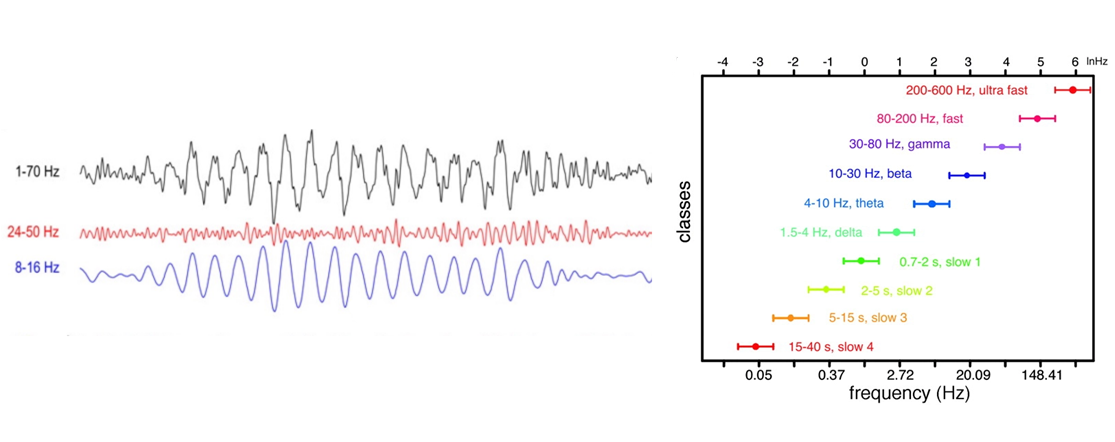
\includegraphics[scale=0.35]{10_5}
    \centering
\end{figure}
From the figure it is also possible to see the different "Brain Bands" or "EEG Bands". The logarithmic scale is due to the fact that the amplitude of EEG 
signals decay following a Power-law behavior: for this reason, the representation is linear in a double-logarithmic scale.

\subsubsection{Oscillations Regulate Neuronal Processing}
Why is important to look at brain oscillations? \\ Neurons communicate with spikes. Also LFPs have possibilities to control the spikes: in this sense, 
oscillations are not just a secondary element of the true activity (and so, in this sense they are not epiphenomena).

\paragraph{Example:}
\begin{figure}[H]
    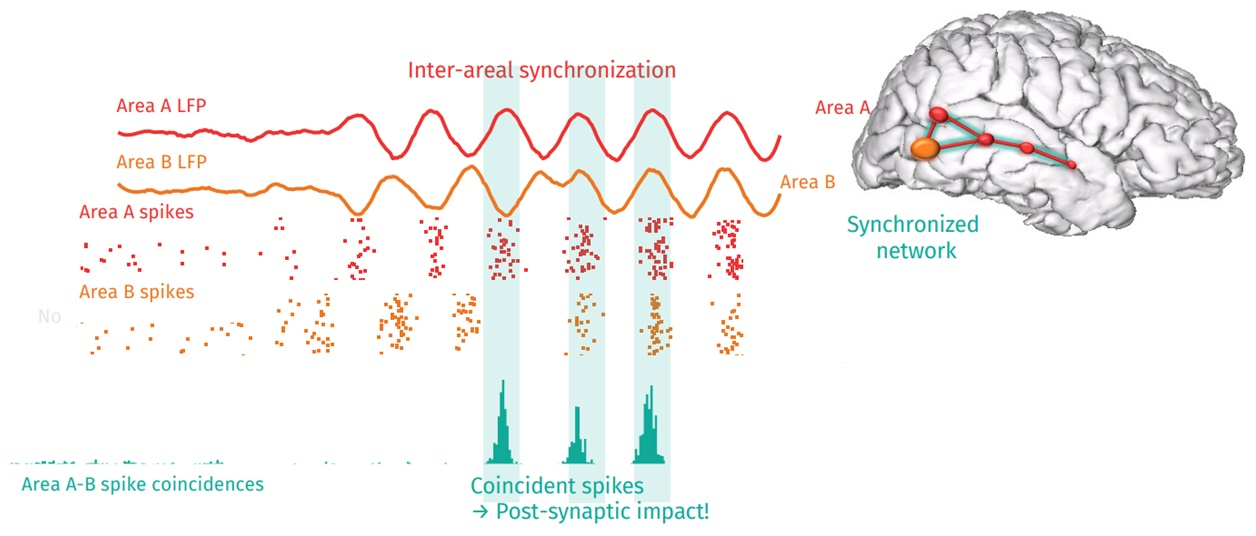
\includegraphics[scale=0.25]{10_6}
    \centering
\end{figure}
In this example two signals are recorded from different brain areas (Area \(A\) and Area \(B\)), having access on both Local Field Potentials and spiking 
activity. When the oscillations of the field potentials of the two regions are in opposite phase, the region which generated the activity (the one that is 
trying to communicate) will be blocked by the fact that the local field potential in the other region has a reduction in voltage, that blocks the voltage-dependent 
channels. If there is a perfect alignment, what happens is exactly the opposite: if one brain region fires, the other responds, and in this case there is \textbf{
communication}, which allows to conclude that \textbf{temporal synchronization between field potentials is supportive for neural activity}.\\
By looking at the LFPs, it is possible to make a link between physiology and cognition.

\subsubsection{Communication Through Coherence Theory}
The hypothesis has been formalized by Fries P., in 2005 and 2015. His theory, called "\textit{Communication through coherence framework}", says that if two populations 
have field activities that are "\textbf{coherent}" in time, (which in the sense of Fries means "synchronized"), when one stimulus reaches one population, the same stimulus 
can reach also the other population. On the other hand, when the two are no aligned, given the fact that the oscillations control the excitation and the excitatory cycle 
of the target cells, the signal will not propagate in the network.
\begin{figure}[H]
    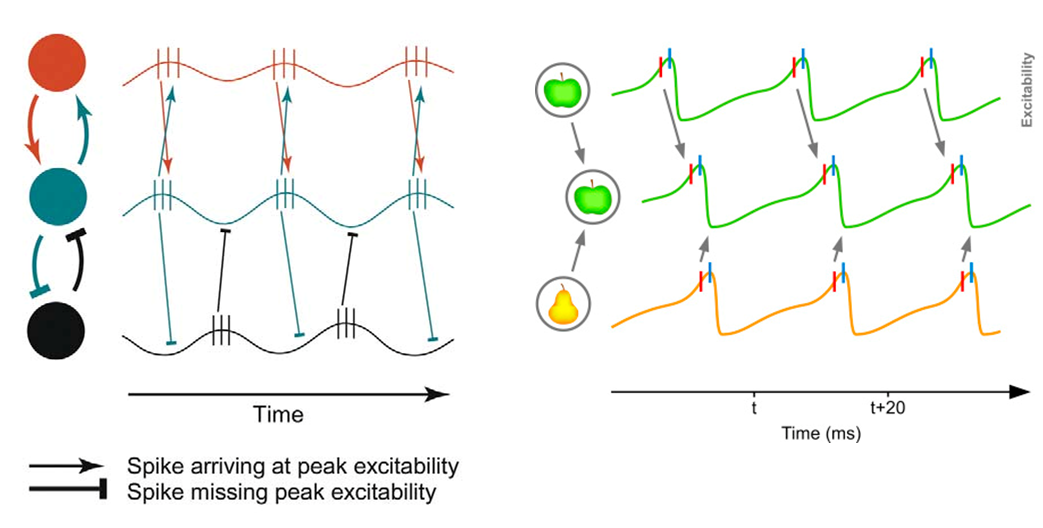
\includegraphics[scale=0.40]{10_7}
    \centering
\end{figure}
This framework applies directly between two neurons, two neuronal ensembles or two brain regions, meaning that 
it's \textbf{scale-free}.
Looking at the second image, if there is a stimulation (first row), this is perceived by all the populations whose 
excitation is perfectly in phase with the first one (in this case, second row). The misalignment of the first two rows 
is consistent considering the distance from the source to the target. For example, Wernicke and Broca, are two brain 
regions responsible on understanding language (Wernicke) and producing language (Broca); 
they are connected by a dense number of axons, and damaging one of the two it could be a problem for the speaking or for understanding language. 
So, it is not important that the oscillations generated in the two regions are perfectly aligned in time, but the important part in this framework is 
that the misalignment (the time delay) is constant, depending on the time that requires one signal to reach the other.\\
On the other hand, if another population (third row) receives a different input and tries to communicate with the central region (row 2), if the excitatory cycle is not 
perfectly aligned, then the activity will be blocked.

\subsubsection{Oscillations Regulate Context Switching}
There are structures that are physically linked (for instance, Wernicke and Broca), and there exists other regions whose connection is more blur (top level networks in the 
cognitive processing) and here there is another kind of behavior, because signals come from very different regions and at the same time. Brain needs to be able to switch 
among different configurations, to process different information very differently but simultaneously, and this happens thanks to brain oscillations, because all brain 
oscillations at all frequency scales exist at the same time.